\documentclass[12pt,a4paper]{article}

\usepackage[T1]{fontenc}
\usepackage[utf8]{inputenc} % Use UTF-8 encoding for input
\usepackage{babel}

\usepackage{lmodern}	
\usepackage{amsmath}
\usepackage{amsfonts}
\usepackage{amssymb}
\usepackage{graphicx}
\usepackage{xcolor}
\usepackage{mathtools}
\usepackage{fancyhdr}
\usepackage{enumitem}
\usepackage{tcolorbox}
\usepackage{colortbl}
\usepackage{multirow}
\usepackage{stmaryrd}
\usepackage{dsfont}
\usepackage{tikz}
\usepackage{hyperref}
\usepackage[upgreek]{txgreeks}
\usepackage{algpseudocode}
\usepackage{algorithm}
\usepackage[text={15cm,24.5cm},centering]{geometry}


% Définir le texte affiché en fin de page
\pagestyle{fancy}
\fancyhf{}  % Clear the default headers and footers
\rfoot{\hrule
    \vspace{0.3cm}
    \noindent\textsf{Learning under physical constraints}
    \hfill \thepage
}
\renewcommand{\headrulewidth}{0pt}

\title{\vspace{4cm}
        Report \\
        \vspace{1cm} \textbf{TP1 : Linear Discriminant Analysis (LDA)} \\ 
        \vspace{4cm} 
}

\author{\textit{Made By} \vspace{0.5cm}\\
        \textbf{Félix Foucher de Brandois}
}
        
\date{\vfill
        \textit{ENSEEIHT} - 
        \textit{Formation ModIA, 5$^{th}$ Year}
        \hfill
        \textit{2024-2025} \\
        \vspace{1cm}
}


\begin{document}

\begin{figure}[t]
    \centering
    
\includegraphics[width=7cm]{src/inp_n7.png}
    \hfill
    
\includegraphics[width=5.5cm]{src/insa_toulouse.png}
\end{figure}


\maketitle
\thispagestyle{empty}

\newpage


\section{Introduction}

The objective of this project is to develop a supervised classifier that can differentiate between various types of numerical simulations of the interstellar medium based on their statistical or spectral properties.
Several sets of simulations were carried out, varying two physical parameters: magnetic field and temperature.
Based on the values of these two parameters, 9 classes were defined. \\
To achieve this classification, the project employs Linear Discriminant Analysis (LDA).



\section{Loading the data}

Images are extracted from binary files arranged by class in folders \texttt{Train} and \texttt{Test}.
Visual examination of the images reveals a complex texture that is difficult to discern with the naked eye.

\begin{figure}[H]
    \centering
    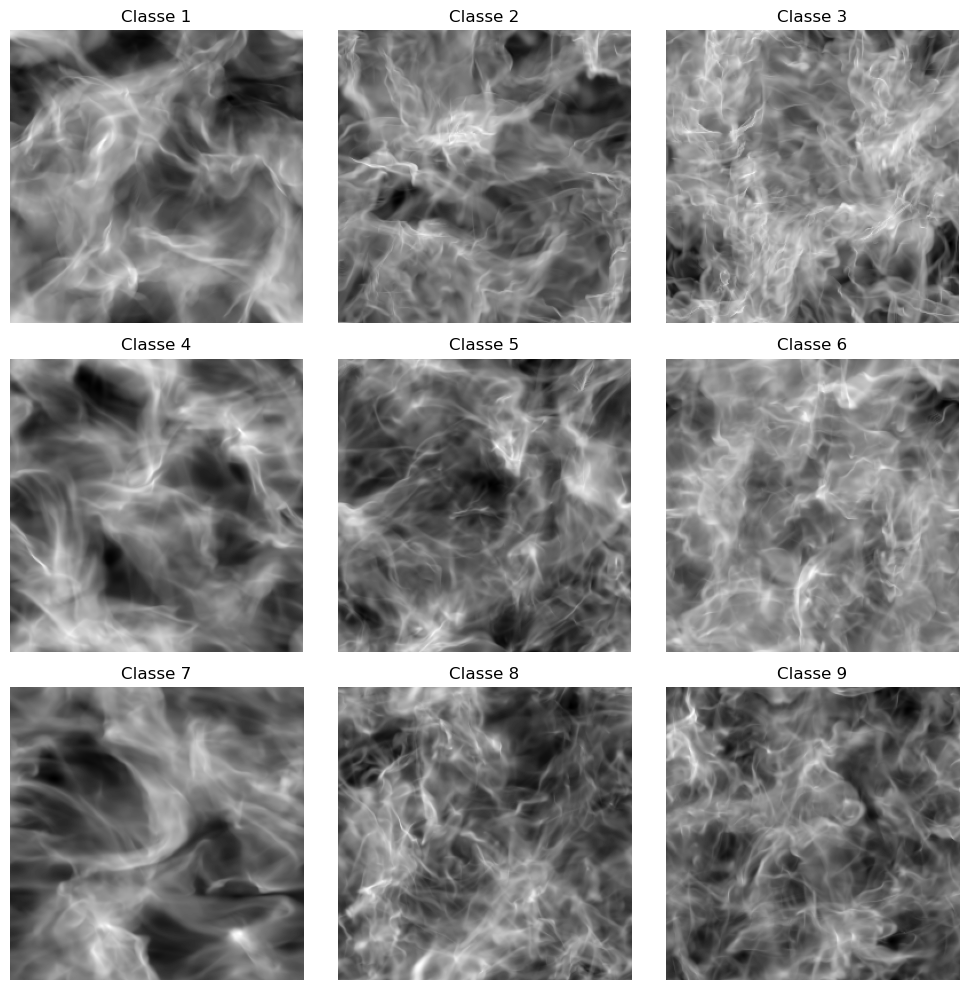
\includegraphics[width=0.97\textwidth]{src/classes.png}
    \caption{Example of images from each class.}
    \label{fig:classes}
\end{figure}

Moreover, we notice that the images have periodic bounding conditions: The left edge is continuous with the right edge, and the top edge is continuous with the bottom edge.

\begin{figure}[H]
    \centering
    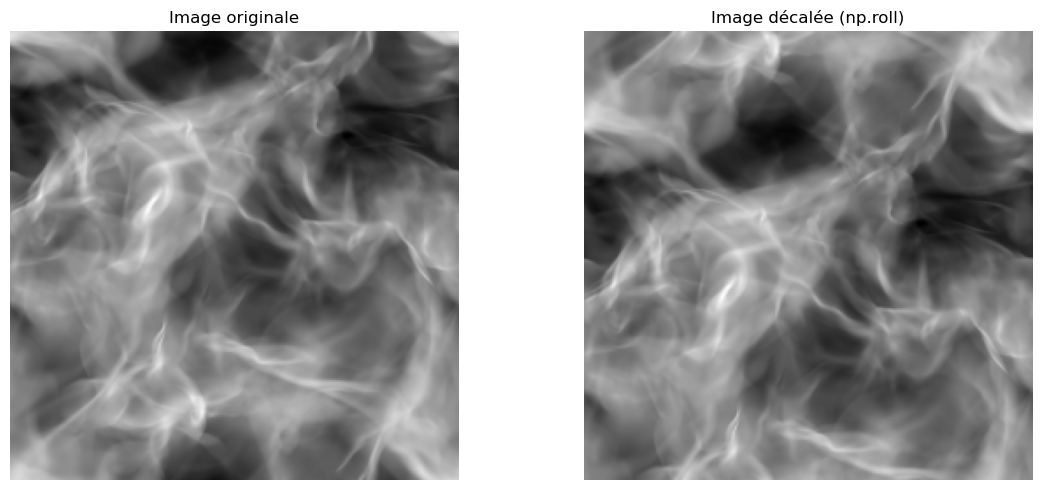
\includegraphics[width=0.8\textwidth]{src/periodic.png}
    \caption{Periodic bounding conditions of the images.}
    \label{fig:periodic}
\end{figure}


\section{Classification with Empirical Mean}

Each image is summarized by the average of its pixels, forming a one-dimensional vector.
Figure \ref{fig:mean} displays the value of the mean for each image, grouped by class.

\begin{figure}[H]
    \centering
    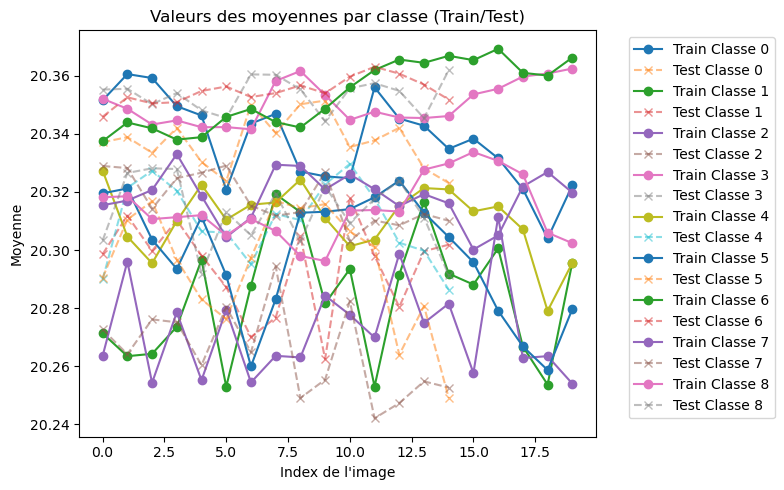
\includegraphics[width=0.9\textwidth]{src/mean.png}
    \caption{Mean of each image, grouped by class.}
    \label{fig:mean}
\end{figure}

The mean values of the images are not sufficient to distinguish between the classes, as they overlap significantly.

We then perform a LDA classification on the mean values of the images to illustrate our intuition. \\

We obtained a classification accuracy of $0.33$ on the training set and $\sim 0.37$ on the test set, which is not satisfactory.
Here is the confusion matrix obtained on the training set:

\begin{figure}[H]
    \centering
    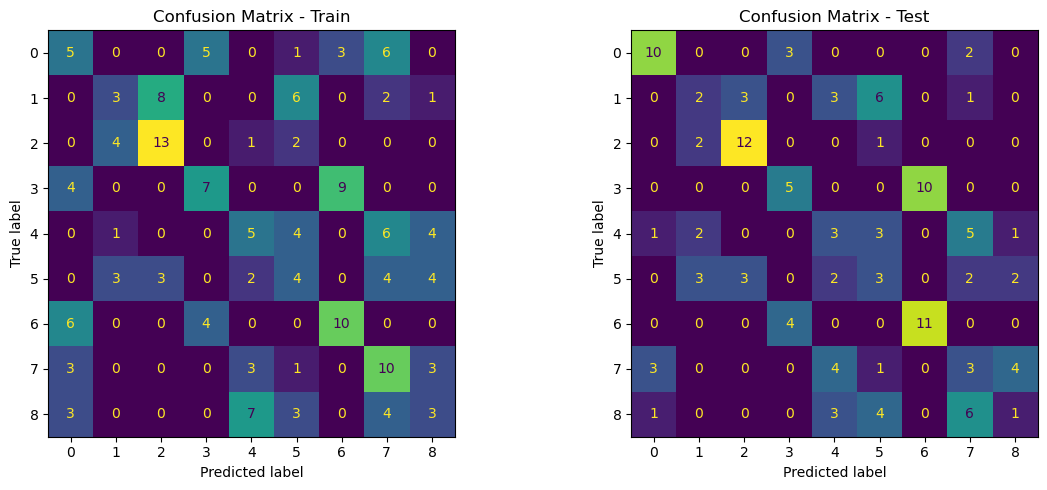
\includegraphics[width=\textwidth]{src/confusion_matrix_mean.png}
    \caption{Confusion matrix of the LDA classification on the mean values of the images.}
    \label{fig:confusion_matrix_mean}
\end{figure}

The confusion matrix shows that the classes are not well separated, with many misclassifications both in the training and test sets.
The mean values of the images do not provide enough information to distinguish between the classes, as they overlap significantly.


\section{Classification with Autocovariance Matrix}

To improve classification performance, we use the spatial autocovariance matrix of each image as a feature descriptor.
The autocovariance matrix is computed as follows: \\

Given an image $X(u)$, where $u$ is a pixel coordinate, the autocovariance for a displacement $\tau = (\tau_1, \tau_2)$ is defined as:
\begin{equation}
    \phi(u, \tau) = \mathbb{E} [(X(u)-\mu_u)(X(u-\tau)-\mu_{u-\tau})]
\end{equation}

where $\mu_u$ is the mean of the image at pixel $u$ and $\mathbb{E}$ denotes the expectation operator (which can be approximated by averaging over all pixels in the image). \\

In our case, the process is assumed stationary, meaning that the autocovariance $\phi(u, \tau)$ depends only on the displacement $\tau$ and not on the specific pixel $u$.
The autocovariance is therefore a matrix defined as:
\begin{equation}
    \Phi(\tau) = \mathbb{E} [(X(u)-\mu)(X(u-\tau)-\mu)]
\end{equation}

with $\tau_1 \in \llbracket 0, d_n \rrbracket$ and $\tau_2 \in \llbracket -d_n, d_n \rrbracket$.
For a chosen displacement range $d_n$, the autocovariance matrix has shape $(d_n + 1) \times (2d_n + 1)$. \\

\newpage

We computed the autocovariance matrix for various values of $d_n \in \llbracket 0, 8 \rrbracket$.
The figure \ref{fig:accuracy_dn} shows the classification accuracy on the training and test sets as a function of $d_n$.
\begin{figure}[H]
    \centering
    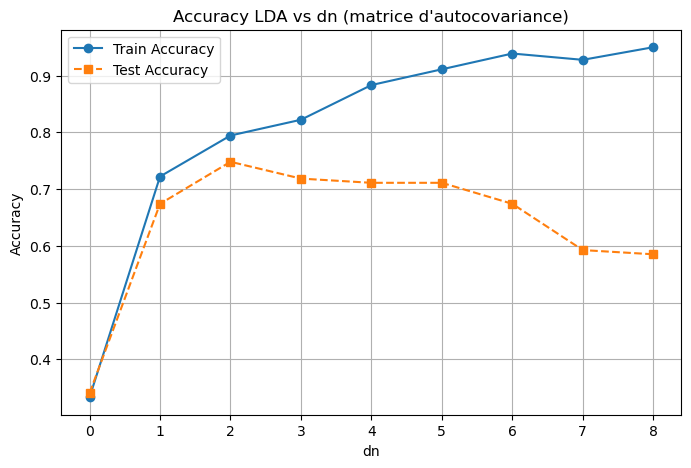
\includegraphics[width=0.7\textwidth]{src/accuracy_dn.png}
    \caption{Classification accuracy on the training and test sets as a function of $d_n$.}
    \label{fig:accuracy_dn}
\end{figure}

The classification accuracy increases for the training set as $d_n$ increases, reaching a maximum of $0.95$ for $d_n = 8$.
However, the accuracy on the test set does not follow the same trend, peaking at $d_n = 2$ with an accuracy of $0.75$.
This suggests that the model is overfitting the training data as $d_n$ increases, capturing noise rather than meaningful patterns. \\

The following figure \ref{fig:confusion_matrix_dn} shows the confusion matrix obtained for $d_n = 8$ on the training and test sets.
\begin{figure}[H]
    \centering
    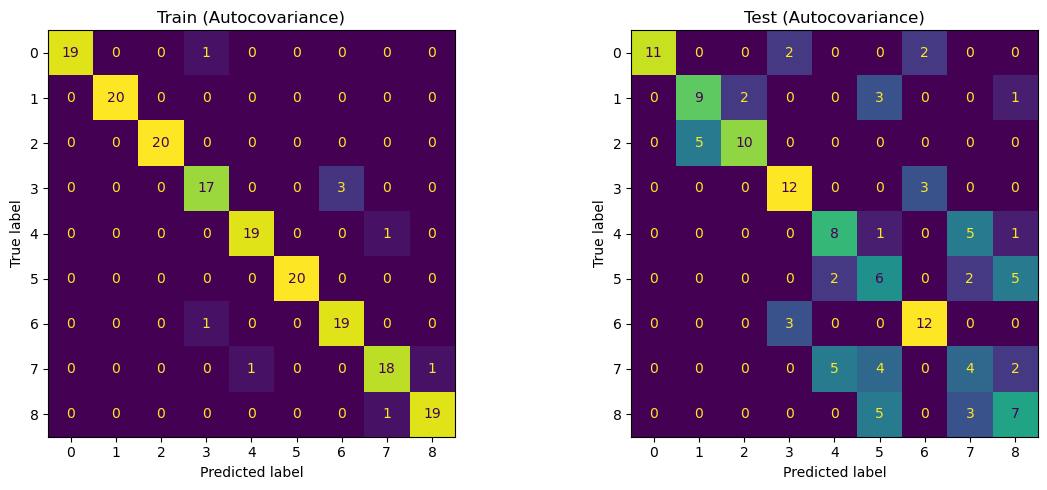
\includegraphics[width=0.9\textwidth]{src/confusion_matrix_dn.png}
    \caption{Confusion matrix of the LDA classification on the autocovariance matrix with $d_n = 8$.}
    \label{fig:confusion_matrix_dn}
\end{figure}

The confusion matrix shows that autocovariance matrices yield much more diagonal confusions matrices and much higher classification accuracy than the mean values.


\section{Classification with Power Spectrum}

To capture global spatial patterns in the frequency domain, we compute the power spectrum of each image using the 2D Fourier Transform.
The power spectrum is defined as the squared magnitude of the Fourier transform:
\begin{equation}
    P(f) = |\mathcal{F}\{X(u)\}|^2
\end{equation}

where $\mathcal{F}\{X(u)\}$ is the Fourier transform of the image $X(u)$.

Note that we have the following relationship between the autocovariance matrix and the power spectrum:
\begin{equation}
    P(f) = \mathcal{F}\{\Phi(\tau)\}
\end{equation}

For each image, we compute the 2D Fourier Transform and extract a square of size $(2 dom + 1) \times (2 dom + 1)$ around the center, where $dom$ is the size of the domain we want to consider.
\begin{figure}[H]
    \centering
    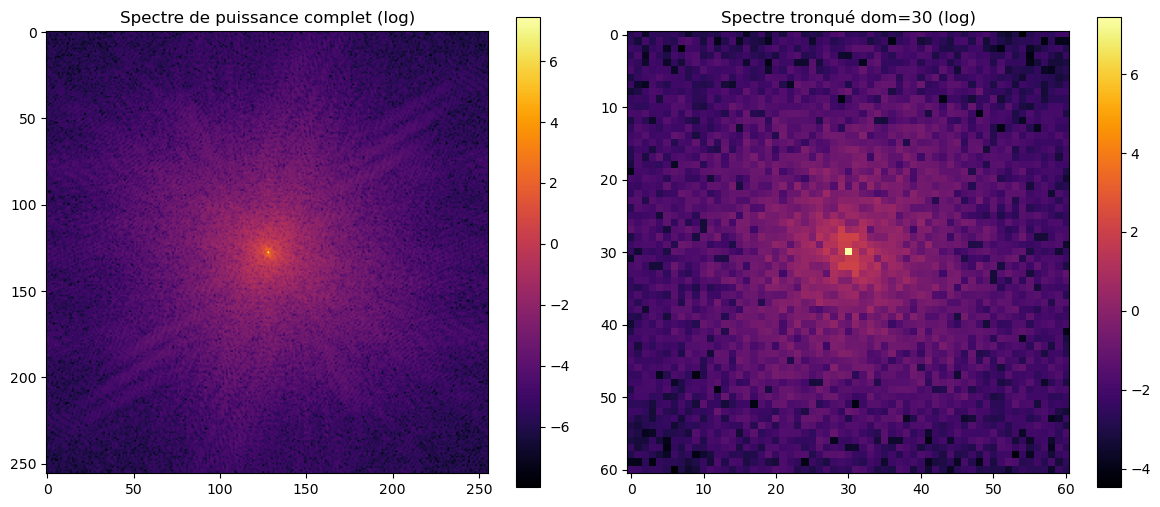
\includegraphics[width=0.9\textwidth]{src/power_spectrum.png}
    \caption{Power spectrum of an image truncated to a domain of size $dom = 30$.}
    \label{fig:power_spectrum}
\end{figure}

We tested several values of $dom \in \llbracket 10, 110 \rrbracket$.
The figure \ref{fig:accuracy_dom} shows the classification accuracy on the training and test sets as a function of $dom$.
\begin{figure}[H]
    \centering
    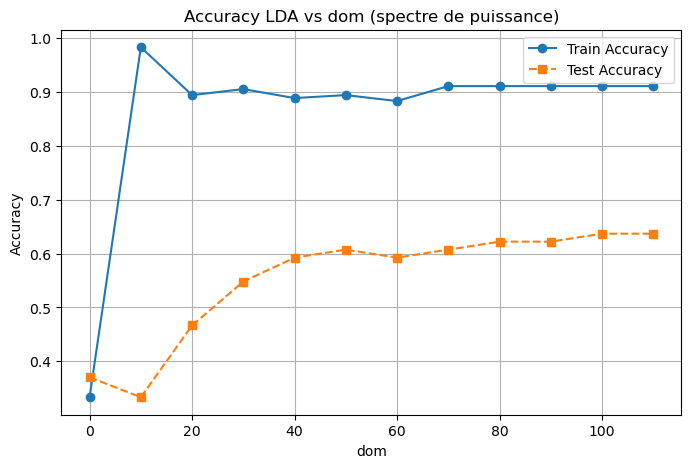
\includegraphics[width=0.7\textwidth]{src/accuracy_dom.png}
    \caption{Classification accuracy on the training and test sets as a function of $dom$.}
    \label{fig:accuracy_dom}
\end{figure}

The classification accuracy is almost constant for the training set, around $0.90$.
However, the accuracy on the test set increases and stabilizes around $0.65$ for $dom \geq 50$.

This suggests that the power spectrum captures relevant global spatial patterns, but the model may not be able to generalize well to unseen data.

\section{Performance analysis}
The following table summarizes the classification accuracy on the training and test sets for the different feature descriptors used:
\begin{table}[H]
    \centering
    \begin{tabular}{|c|c|c|}
        \hline
        Feature Descriptor & Training Accuracy & Test Accuracy \\
        \hline
        Mean Values & 0.33 & 0.37 \\
        Autocovariance Matrix ($d_n = 8$) & 0.95 & 0.59 \\
        Power Spectrum ($dom = 110$) & 0.90 & 0.65 \\
        \hline
    \end{tabular}
    \caption{Classification accuracy for different feature descriptors.}
    \label{tab:performance}
\end{table}

The results show that the autocovariance matrix provides the best performance on the training set, but it does not generalize well to the test set, indicating overfitting.
The power spectrum provides a good balance between training and test accuracy.
The mean is clearly insufficient: it fails to capture the internal structure of the image. \\

In the following figures, we plot the feature vectors (mean, covariance, power spectrum) per class and include their intra-class variance.
\begin{figure}[H]
    \centering
    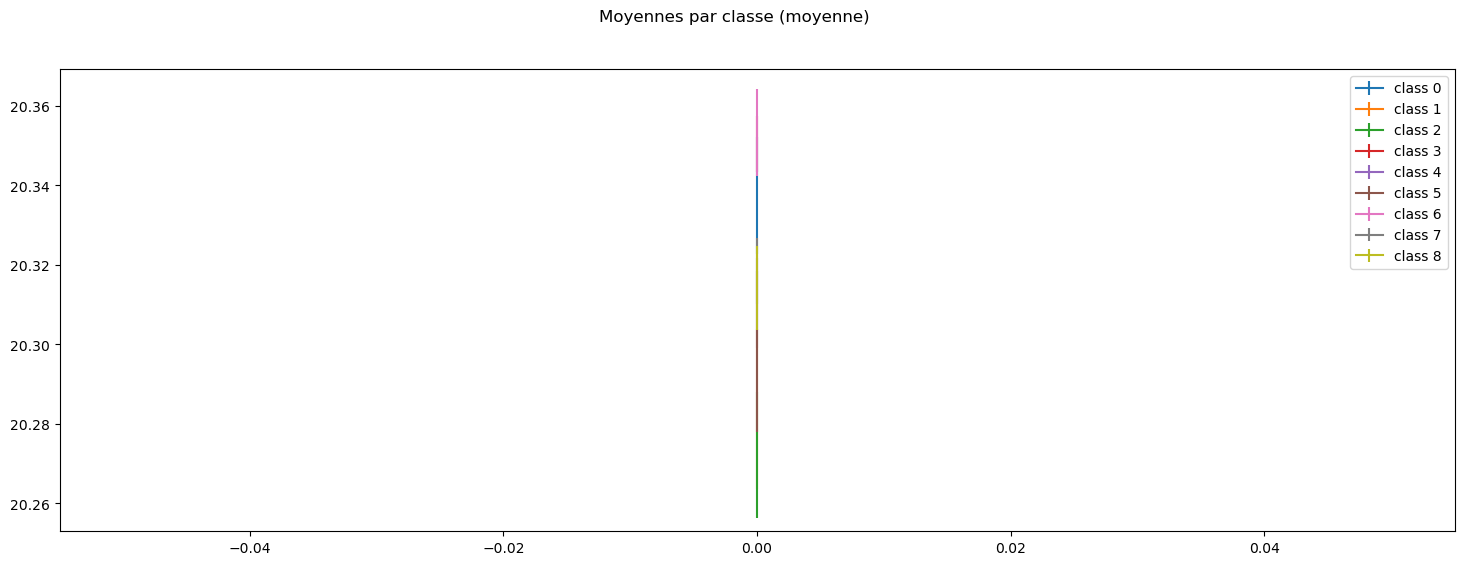
\includegraphics[width=0.8\textwidth]{src/mean_per_class.png}
    \caption{Mean values per class with intra-class variance.}
    \label{fig:mean_per_class}
\end{figure}
\begin{figure}[H]
    \centering
    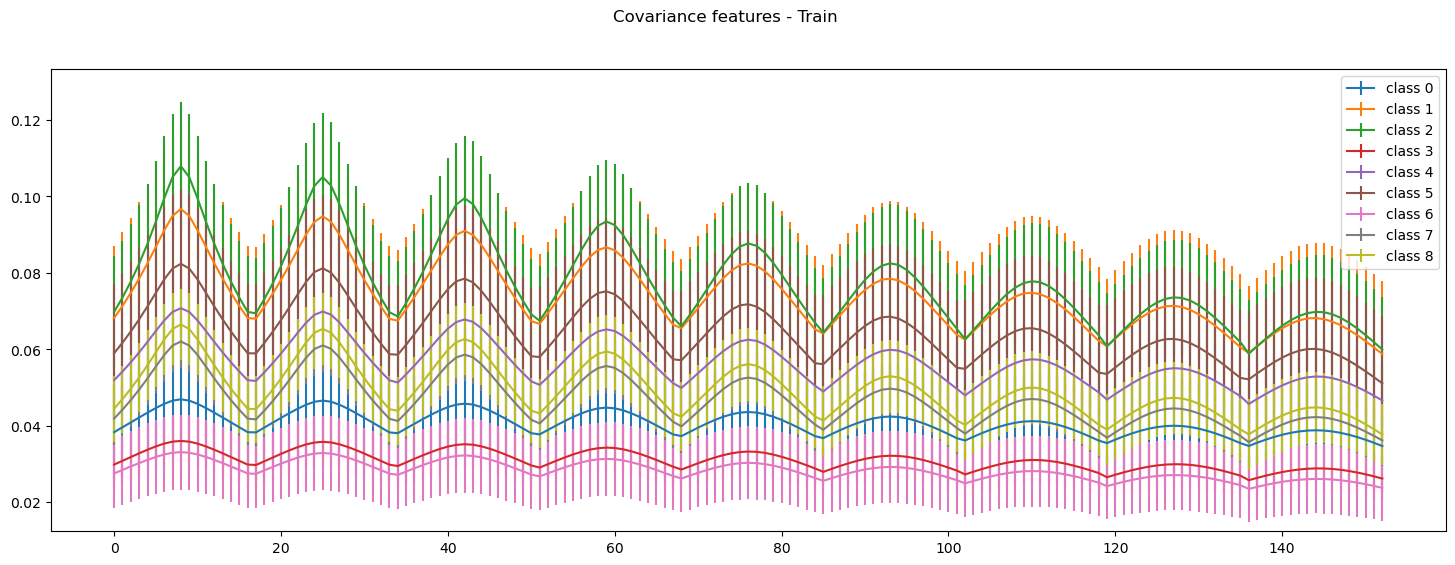
\includegraphics[width=0.8\textwidth]{src/autocovariance_per_class.png}
    \caption{Autocovariance matrices per class with intra-class variance.}
    \label{fig:autocovariance_per_class}
\end{figure}
\begin{figure}[H]
    \centering
    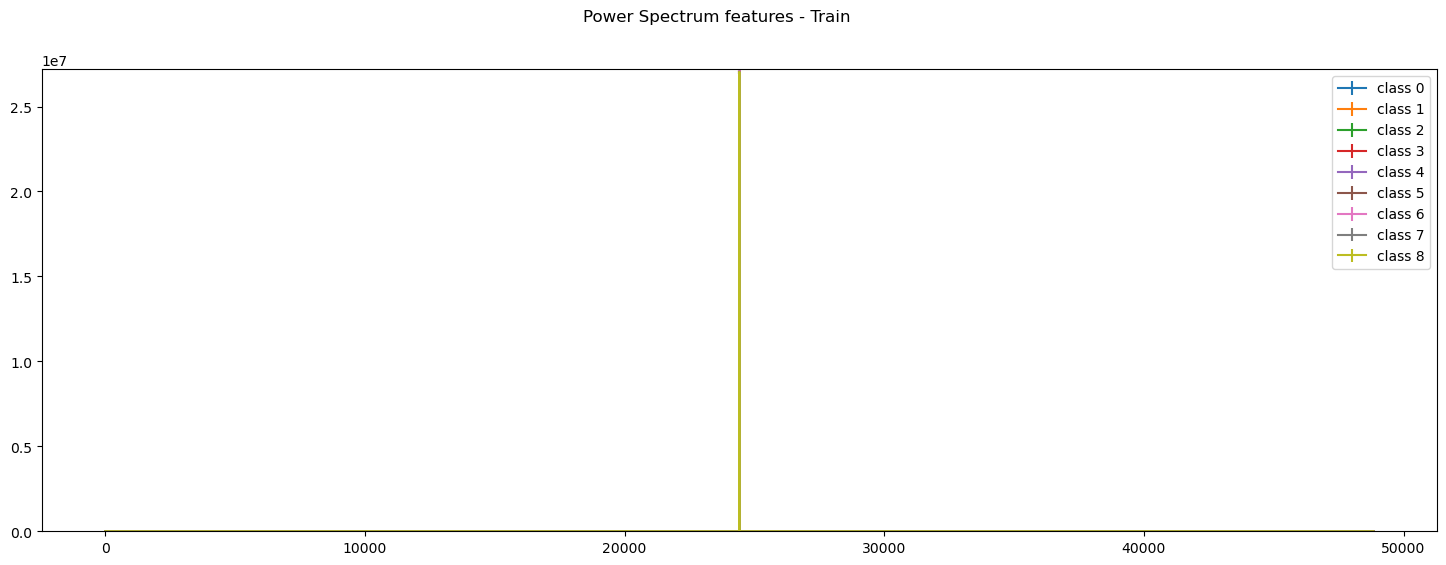
\includegraphics[width=0.8\textwidth]{src/power_spectrum_per_class.png}
    \caption{Power spectra per class with intra-class variance.}
    \label{fig:power_spectrum_per_class}
\end{figure}

This illustrates the separation between classes for each feature descriptor.
We observe that the mean values do not provide sufficient separation between classes, while the autocovariance matrices show more distinct patterns.

\section{Conclusion}
In this project, we explored different feature descriptors for classifying images of the interstellar medium based on their statistical properties.
We found that the mean values of the images are not sufficient for classification, as they do not capture the internal structure of the images.
The autocovariance matrix provides better performance on the training set, but it does not generalize well to the test set, indicating overfitting.
The power spectrum captures relevant global spatial patterns and provides a good balance between training and test accuracy. \\
Future work could explore other group invariant features such as the rotation invariant.


\end{document}